\documentclass[12pt]{article}
 
\usepackage[margin=1in]{geometry} 
\usepackage{amsmath,amsthm,amssymb}
\usepackage{hyperref}
\usepackage{graphicx}
\usepackage{xcolor}
\usepackage[many]{tcolorbox}
\tcbuselibrary{listings}
\usepackage{listings}
\usepackage{float}

\definecolor{lg}{HTML}{f0f0f0}

\newtcblisting{pycode}{
    colback=lg,
    boxrule=0pt,
    arc=0pt,
    outer arc=0pt,
    top=0pt,
    bottom=0pt,
    colframe=white,
    listing only,
    left=15.5pt,
    enhanced,
    listing options={
        basicstyle=\small\ttfamily,
        keywordstyle=\color{blue},
        language=Python,
        showstringspaces=false,
        tabsize=2,
        numbers=left,
        breaklines=true
    },
    overlay={
        \fill[gray!30]
        ([xshift=-3pt]frame.south west)
        rectangle
        ([xshift=11.5pt]frame.north west);
    }
}

\lstset{
    language=Python,
    basicstyle=\small\ttfamily,
}

 
\begin{document}
 
\title{Exercise 4}
\author{Cristian Manuel Abrante Dorta - 888248\\
ELEC-E8125 - Reinforcement Learning}

\maketitle
\section{Approximation with non-linear features}

\subsection{Task 1}
\textbf{Implement Q-learning using function approximation, at every timestep using the latest state transition to perform a TD(0) update. Test the implementation on the
Cartpole environment. Test two different features for state representations}\\

For the implementation of function approximation using TD(0) update, the following formula was used for updating the target ($\delta$) values of the stochastic gradient regressor:

\begin{equation}
    \delta = r + \gamma \cdot max_a {Q(\phi(s'), a)}
\end{equation}

Where:

\begin{itemize}
    \item $r$: is the reward obtained in the current state.
    \item $\gamma$: is the discount factor for future actions.
    \item $\phi(s)$: is the featurizer function, in this task two different functions were used.
    \item $max_aQ(\phi(s'), a)$: is the maximum value function of the next state, following the optimal policy.
\end{itemize}

Using this formula, and for the two featurizer functions, the following plots were obtained:

\begin{figure}[H]
    \centering
   \begin{minipage}{0.48\textwidth}
     \centering
     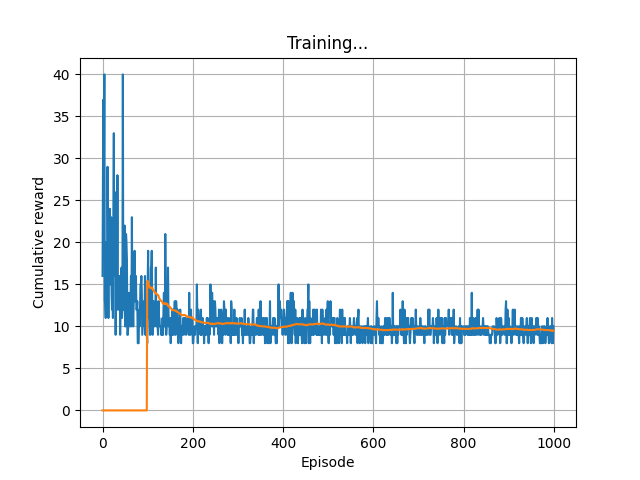
\includegraphics[width=0.9\linewidth]{exercise-4/plots/task-1a.png}
     \caption{Plot for handcrafted feature vector}
     \label{fig:task-2-1}
   \end{minipage}\hfill
   \begin{minipage}{0.48\textwidth}
     \centering
     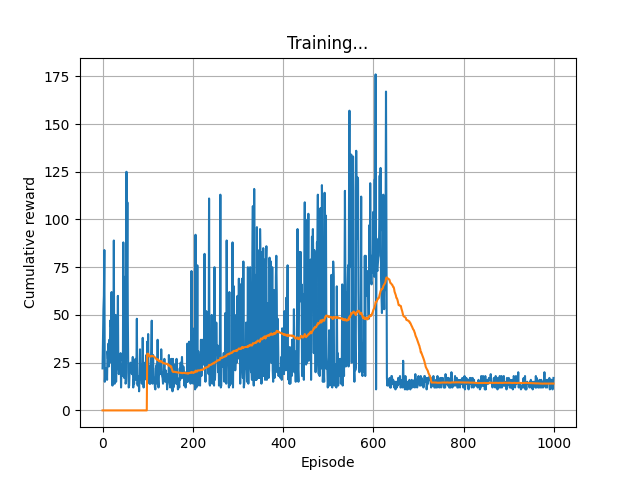
\includegraphics[width=0.9\linewidth]{exercise-4/plots/task-1b.png}
     \caption{Plot for radial basis function representation}
     \label{fig:task-2-2}
   \end{minipage}
\end{figure}

As we can see in this plots, the second function allows the agent to actually learn the underlying pattern, on the contrary, using the first feature vector, the model is not able to learn. 

\subsection{Question 1}
\textbf{
Would it be possible to learn accurately Q-values for the Cartpole problem using linear features (by passing the state directly to a linear regressor)? Why/why not?
}\\

There are some reasons that would make difficult to learn accurately the Q-values for the Cartpole environment if we pass directly the state to the linear regressor. \\

The main drawback of doing this, is that the state is not scaled by default, and that would make more difficult for the regressor to learn the weights. For overcoming this first difficulty, the value of the states has been scaled using an standard scaler, fitted with an arbitrary dataset created with a range of possible values. \\

The second drawback of passing the state directly is that it only contains 4 values, so the regressor would only have four weights for features. This could be not enough information for the generalization of the Q values.

\subsection{Task 2}
\textbf{Modify your Task 1 implementation to perform minibatch updates and use experience replay (while keeping the original code for Task 1 submission). Run the experiments with Cartpole with both feature representations.}\\

Using minibatch updates and experience replay, Task 1 was executed, obtaining the following plots as a result:

\begin{figure}[H]
    \centering
   \begin{minipage}{0.48\textwidth}
     \centering
     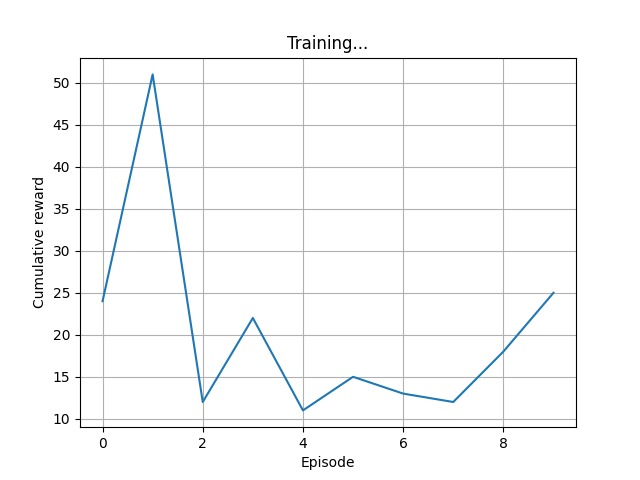
\includegraphics[width=0.9\linewidth]{exercise-4/plots/task-2a.png}
     \caption{Minibatch and experience replay with handcrafted vector}
     \label{fig:task-2-1}
   \end{minipage}\hfill
   \begin{minipage}{0.48\textwidth}
     \centering
     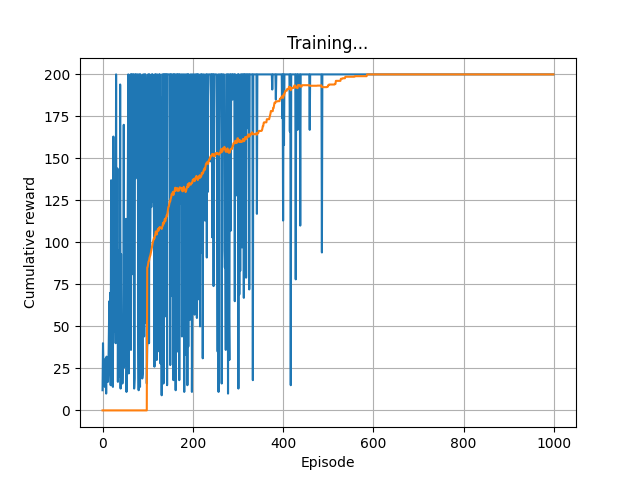
\includegraphics[width=0.9\linewidth]{exercise-4/plots/task-2b.png}
     \caption{Minibatch and experience replay with radial basis function representation}
     \label{fig:task-2-2}
   \end{minipage}
\end{figure}

\section{Task 2}
To embed code snippets in the report, you can use the \texttt{pycode} environment.

\begin{pycode}
for episode_number in range(train_episodes):
    reward_sum, timesteps = 0, 0
    done = False
    # Reset the environment and observe the initial state
    observation = env.reset()

    # Loop until the episode is over
    while not done:
        # Get action from the agent
        action, action_probabilities = agent.get_action(observation)
        previous_observation = observation

        # Perform the action on the environment, get new state and reward
        observation, reward, done, info = env.step(action)

        # Store action's outcome (so that the agent can improve its policy)
        agent.store_outcome(previous_observation, action_probabilities, action, reward)

        # Draw the frame, if desired
        if render:
            env.render()
\end{pycode}

\section{Question 1}

If you add a figure, you can refer to it using Figure.~\ref*{fig:fig1}.

\begin{figure}[h] 
	\centering  % Remember to centre the figure
    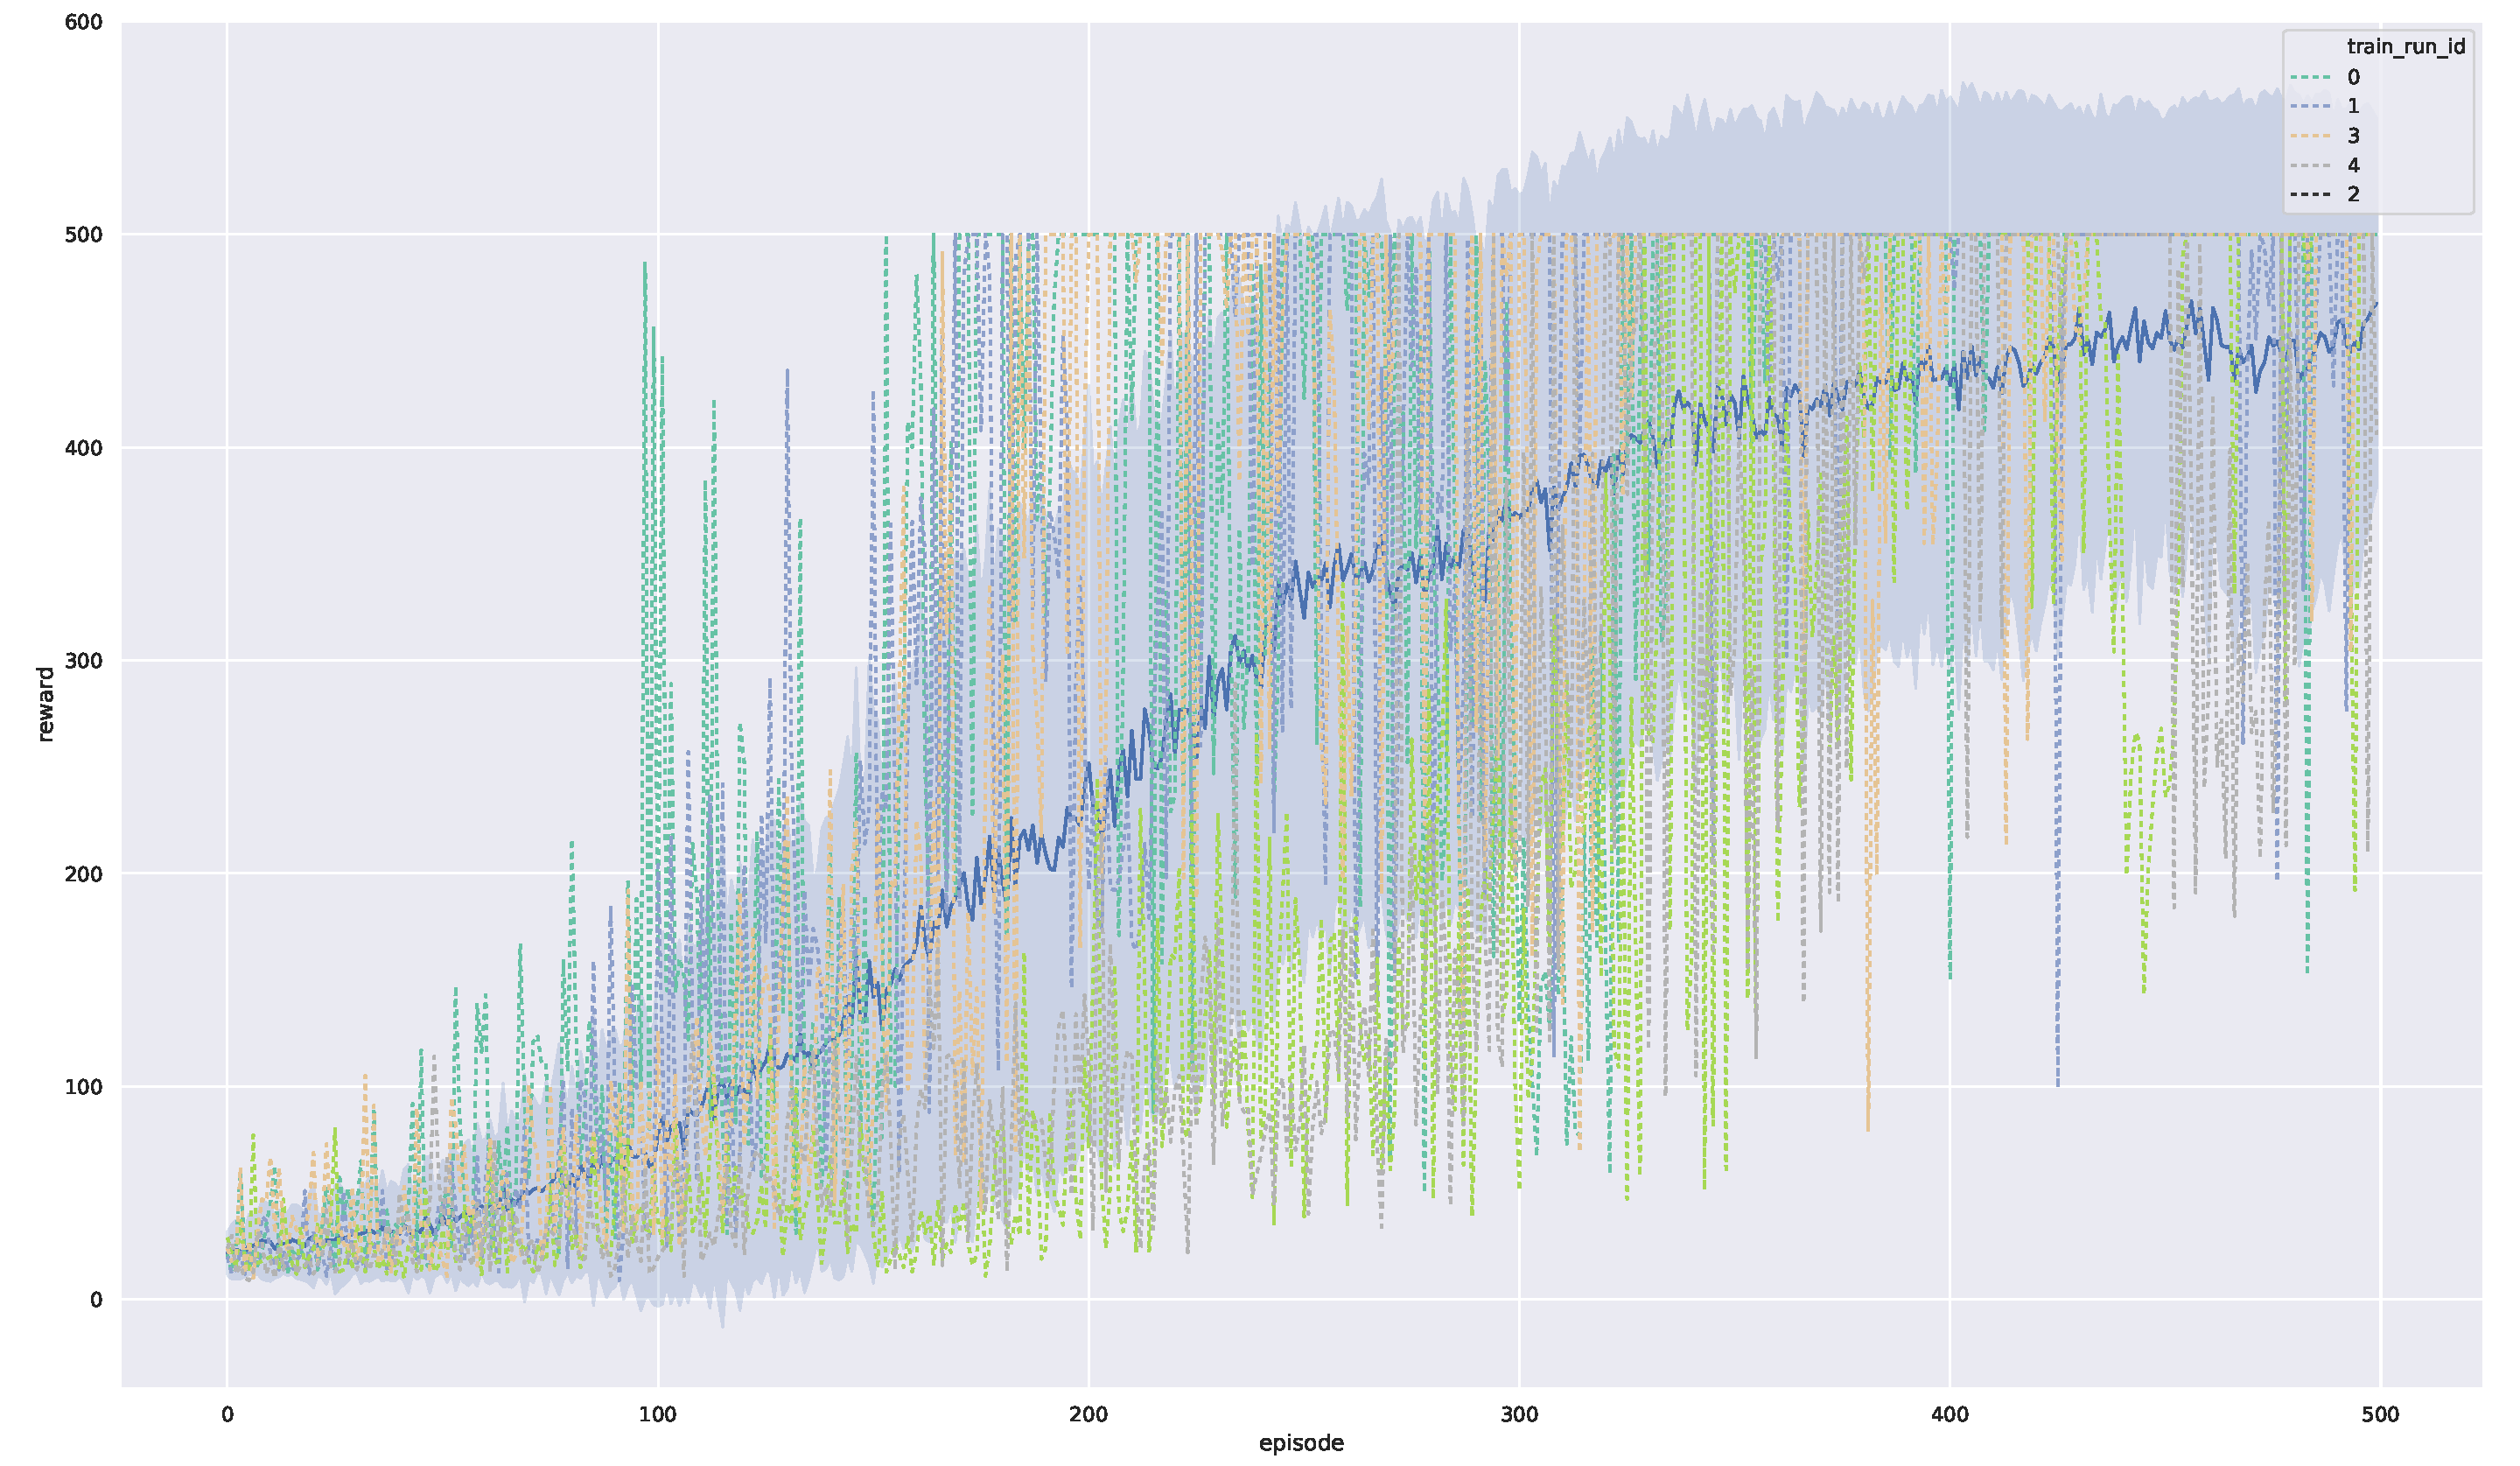
\includegraphics[width=0.9\columnwidth]{img/training.pdf}
	\caption{This is a sample figure.}
	\label{fig:fig1}
\end{figure}

\bibliographystyle{ieeetr}
\bibliography{template}  % Modify template with your bibliography name
\end{document}
